\documentclass[../rapport_MVEX01-11-05]{subfiles}
\begin{document}
\subsubsection{Egenskaper}
En Hidden Markov Model behöver observationer för att fungera; dessa
observationer kommer vi att identifiera med hjälp av klassificering av
nyckelbilder ur videon utifrån ett antal egenskaper vi identifierar
med hjälp av den binära hudkartan för motsvarande bild.

För att kunna applicera metoden även vid stora variationer --- olika
personer, avstånd till kameran, uppställningar osv. --- är det viktigt
att endast använda egenskaper som är oberoende av sådana variabler.
Position och absolut storlek är exempel på egenskaper som inte bör
användas, eftersom dessa kan variera mycket även inom en specifik
gest. Hastighet kan räknas in i denna grupp men måste ändå användas
om rörelsegester ska kunna identifieras.

Många av egenskaperna som beskrivs här kan beräknas effektivt av
\MATLAB-kommandot \texttt{regionprops}.

\paragraph{Inledande definitioner}

För beräkning av vissa egenskaper behöver man definiera två
grundläggande begrepp; den inneslutande lådan och centroiden. Dessa
två kan användas för att i någon mening hitta ''mitten'' av objektet
vi undersöker. Den inneslutande lådan kan dessutom användas för vissa
jämförelser relaterade till area (dvs. densitetsliknande begrepp).

\subparagraph{Inneslutande låda}

Den inneslutande lådan är den minsta rektangeln som innehåller hela
objektet. Denna kan effektivt beräknas genom att lokalisera
extrempunkterna i $x$- och $y$-led, dvs. de punkter närmst kanterna
som är en del av objektet. Lådan har fyra egenskaper: bredd, höjd samt
position i $x$- och $y$-led. Utifrån dessa kan vi även beräkna en femte
och sjätte egenskap; mittpunkt i $x$- och $y$-led:

\begin{gather*}
  \textrm{Box}_{cx}(A) = \textrm{Box}_x(A) + \textrm{Box}_w(A)/2\\
  \textrm{Box}_{cy}(A) = \textrm{Box}_y(A) + \textrm{Box}_h(A)/2
\end{gather*}

\subparagraph{Centroid}

Centroiden är masscentrum för området, och beräknas enligt

\begin{equation*}
  \textrm{centroid}(A) = \left\lfloor\frac{
    \sum\limits_{a\in A}m_a\vec{r}_a
  }{
    \sum\limits_{a\in A}m_a
  }\right\rfloor =
  \left\lfloor\sum\limits_{a\in
  A}\frac{\vec{r}_a}{\textrm{Area}(A)}\right\rfloor,
\end{equation*}

där man använder att $m_a=1,\:\forall a\in A$ eftersom bilden är
binär ($m_a$ är helt enkelt intensiteten i punkten $a$ och
$\vec{r}_a$ är positionen av punkten $a$). Operatorn $\lfloor
x\rfloor$ avrundar $x$ nedåt till närmsta heltal. Centroiden är vektorvärd,
med ett $x$- och ett $y$-element.

\paragraph{Hu-moment}

Dessa moment definierades först av \citeasnoun{Hu62} och är ett försök att
göra centralmomenten rotations-, skalnings- och translationsinvarianta och
därmed mer användbara. Sju Hu-moment definieras \cite[s.~185]{Hu62}:

\begin{align*}
	I_1 =& \;\mu_{20} + \mu_{02}\\
	I_2 =& \left(\mu_{20} - \mu_{02}\right)^2 + 4\mu^2_{11}\\
	I_3 =& \left(\mu_{30} - 3\mu_{12}\right)^2 +
	       \left(3\mu_{21} - \mu_{03}\right)^2\\
	I_4 =& \left(\mu_{30} + \mu{12}\right)^2 +
 	       \left(\mu_{21} + \mu_{03}\right)^2\\
	I_5 =& \left(\mu_{30} - 3\mu_{12}\right)
	       \left(\mu_{30} + \mu_{12}\right)
	       \left(\left(\mu_{30}+\mu{12}\right)^2 -
	       3\left(\mu{21}+\mu{03}\right)^2\right) + \\
 	    &+ \left(3\mu_{21} - \mu_{03}\right)\left(\mu_{21} + \mu_{03}\right)
	       \left(3\left(\mu_{30} + \mu{12}\right)^2 -
	       \left(\mu_{21} + \mu_{03}\right)^2\right)\\
	I_6 =& \left(\mu_{20}-\mu_{02}\right)
	       \left(\left(\mu_{30}+\mu_{12}\right)^2 -
	       \left(\mu_{21}+\mu_{03}\right)^2\right) + \\
	    &+ 4\mu_{11}\left(\mu_{30}+\mu_{12}\right)
	       \left(\mu_{21}+\mu_{03}\right)\\
	I_7 =& \left(3\mu_{21}-\mu_{03}\right)\left(\mu_{30}-\mu_{12}\right)
	       \left(\left(\mu_{30}+\mu_{12}\right)^2 - 
	       3\left(\mu_{21}+\mu_{03}\right)^2\right) - \\
	    &- \left(\mu_{30} - 3\mu_{12}\right)\left(\mu_{21}+\mu_{03}\right)
	       \left(3\left(\mu_{30}+\mu_{12}\right)^2 - 
  	     \left(\mu_{21}+\mu_{03}\right)^2\right)
\end{align*}

Ovan är $\mu_{pq}$ centralmomenten, som definieras av

\begin{equation*}
	\mu_{pq} = \sum\limits_x\sum\limits_y
	           \left(x-\bar{x}\right)^p
	           \left(y-\bar{y}\right)^q
	           f(x,y)
\end{equation*}

där $\bar{x}$ och $\bar{y}$ är centroidens x- och y-komponent, och $f(x,y)$ är
bildens ljusstyrka. I vårt fall gäller att $f\mapsto\left\{0,1\right\}$
eftersom bilden är binär.

\paragraph{Konvexitet}

Konvexitet \cite[s.~26]{Rudemo09} är ett användbart dimensionslöst
mått som i någon mening beskriver hur konvext ett objekt är --- för
gestigenkänning är detta ett relevant mått på huruvida fingrarna är
utsträckta eller inte, men även på om de sitter tätt ihop (ex.
stopptecken) eller löst konfigurerade (ex. segertecken). Det
definieras av

\begin{equation*}
  \textrm{konvexitet}(A) = \frac{\left|\partial A_h\right|}{\left|\partial A\right|}
\end{equation*}

där $A_h$ är det konvexa skalet till $A$ (dvs. det minsta konvexa område som
helt täcker $A$) och $\partial A$ betecknar randen till $A$ (i diskret
mening).

\paragraph{Kompakthet}

Kompakthet \cite[s.~26]{Rudemo09} är ännu ett dimensionslöst mått som
beskriver hur kompakt ett objekt är.
Cirkeln är det mest kompakta objektet, och ju fler irregulariteter
randen innehåller desto mindre blir kompaktheten. Kompakthet
definieras av

\begin{equation*}
  \textrm{kompakthet}(A) = \frac{\textrm{Area}(A)}{\left|\partial
  A\right|^2}.
\end{equation*}

\paragraph{Soliditet}
\label{feat:soliditet}

Soliditet är i någon mening ett mått på hur poröst ett objekt är. Det
definieras av ration mellan objektets area och det konvexa skalets
area enligt

\begin{equation*}
  \textrm{soliditet}(A) = \frac{\textrm{Area}(A)}{\textrm{Area}(A_h)},
\end{equation*}

och är därför dimensionslöst. Detta mått kan vara mycket hjälpsamt för
gester som t.ex.~''OK'' (en ring formad av tumme och pekfinger, med
övriga fingrar riktade uppåt).

\paragraph{Fyrkantighet}
\label{feat:fyrkantighet}

Den här egenskapen är helt enkelt ett mått på hur kvadratisk den
inneslutande lådan är, och på så sätt mäter det hur ''utsträckt'' en
gest är. Dess definition är mycket enkel:

\begin{equation*}
  \textrm{fyrkantighet}(A) = \frac{\textrm{Box}_w(A)}{\textrm{Box}_h(A)}
\end{equation*}

En perfekt kvadratisk låda har alltså fyrkantighet $1$, och ju mer
fyrkantigheten avviker från detta värde desto mer avlång är gesten.
Notera dock att detta mått är låst till rutnätet, och att
excentriciteten mäter i princip samma sak men utgår från den
omslutande ellipsen och därmed inte är låst till rutnätet.

\paragraph{Excentricitet}

Excentriciteten är ett mått på hur utsträckt ett objekt är (precis som
fyrkantigheten, \ref{feat:fyrkantighet}), och utgår från den ellips som
vars andramoment är samma som bildens. Excenticiteten definieras av avståndet
mellan andramomenten i ellipsen genom längden av den längsta axeln. Därmed
tar måttet, till skillnad från fyrkantigheten, även hänsyn till vilken vinkel
objektet ligger i gentemot horisontalaxeln.

\paragraph{Utsträckning}

Utsträckningen mäter hur stor del av den inneslutande lådan som
faktiskt täcks av vårt objekt. Egenskapen kan ses som ett alternativ
till soliditeten (\ref{feat:soliditet}) och definieras enligt

\begin{equation*}
  \textrm{utsträckning}(A) =
  \frac{\textrm{Area}(A)}{\textrm{Area}(\textrm{Box}(A))}.
\end{equation*}

\paragraph{Oberoende}

För att kunna utnyttja egenskaperna maximalt är det lämpligt om dessa
inte innehåller redundant information, dvs. att de är någorlunda
oberoende. Några av egenskaperna kan förväntas vara beroende, eftersom
dess definitioner är mycket lika (så är exempelvis fallet med
soliditet och utsträckning), men för att dra konkreta slutsatser om
beroende mellan egenskaper måste en statistisk analys utföras.

\begin{figure}[htbp]
	\centering
	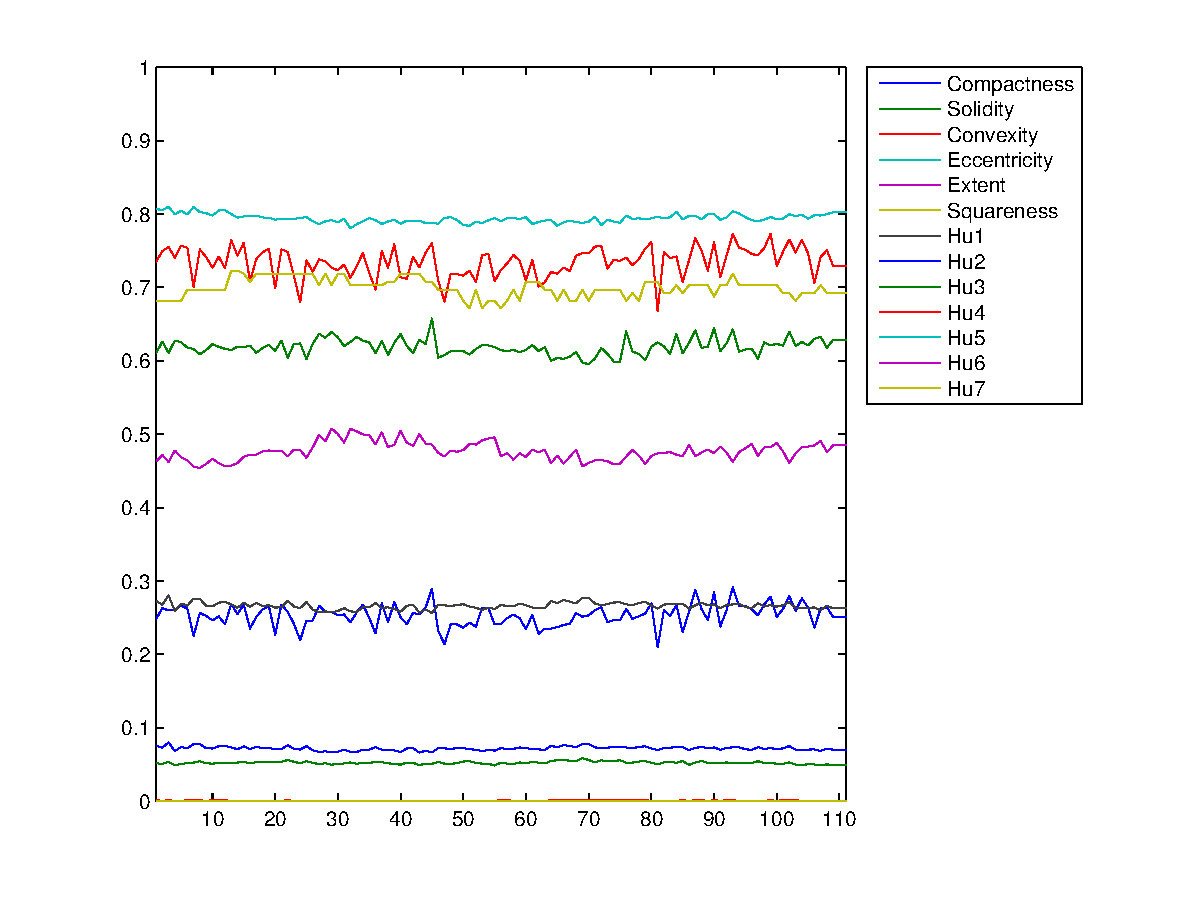
\includegraphics[width=\textwidth]{bilder/feat-move}
	\caption{En statisk gest har som väntat och önskat relativt
	stora korrelationer mellan egenskaperna.}
	\label{fig:featmove}
\end{figure}

Det är självklart lämpligt att egenskaperna inom en gest är beroende;
det visar att egenskaperna är stabila och inte varierar i förhållande
till varandra inom en enskild gest. Dessa syns i
figur~\ref{fig:featmove}, och bekräftas av enkla korrelationstest med
\MATLAB-funktionen \texttt{corrcoef}.

Mellan gester är det dock viktigt att egenskaperna inte är beroende;
detta innebär att vi har redundant information. Ett
\texttt{corrcoef}-test på medelvärden av egenskaperna från flera olika
egenskaper visar, med stor osäkerhet, att det endast är Hu-momenten av
ordning 4--7 som korrelerar mellan gester.

\paragraph{Normalisering}

För att kunna destillera träningsdata till färre observationer och sedan
kunna identifiera testdata enligt dessa på ett bra sätt använder vi
$k$-nearest-neighbour-metoden. Eftersom denna grundar sig på euklidiskt
avstånd över egenskapsrummet är det viktigt att alla egenskaper antar värden
i ungefär samma storleksordning. För att se till att så är fallet är det
lämpligt att normera all indata utifrån konstanter som beräknas genom
normering av träningsdata, lämpligtvis genom att anpassa träningsdatan till en
enkel $N(0,1)$-distribution. Man får då, för varje gest, en
förskjutningsparameter $\mu$ och en skalningsparameter $\sigma$. Dessa kan
användas för att senare normalisera indata:

\begin{equation*}
	\hat{x} = \frac{x - \mu_x}{\sigma_x}
\end{equation*}

\paragraph{Observerade värden}

Ny figur med endast de statiska gesterna, förklara vilka som ser ut
att fungera bäst för att urskilja gester.

\begin{figure}[htbp]
  \centering
  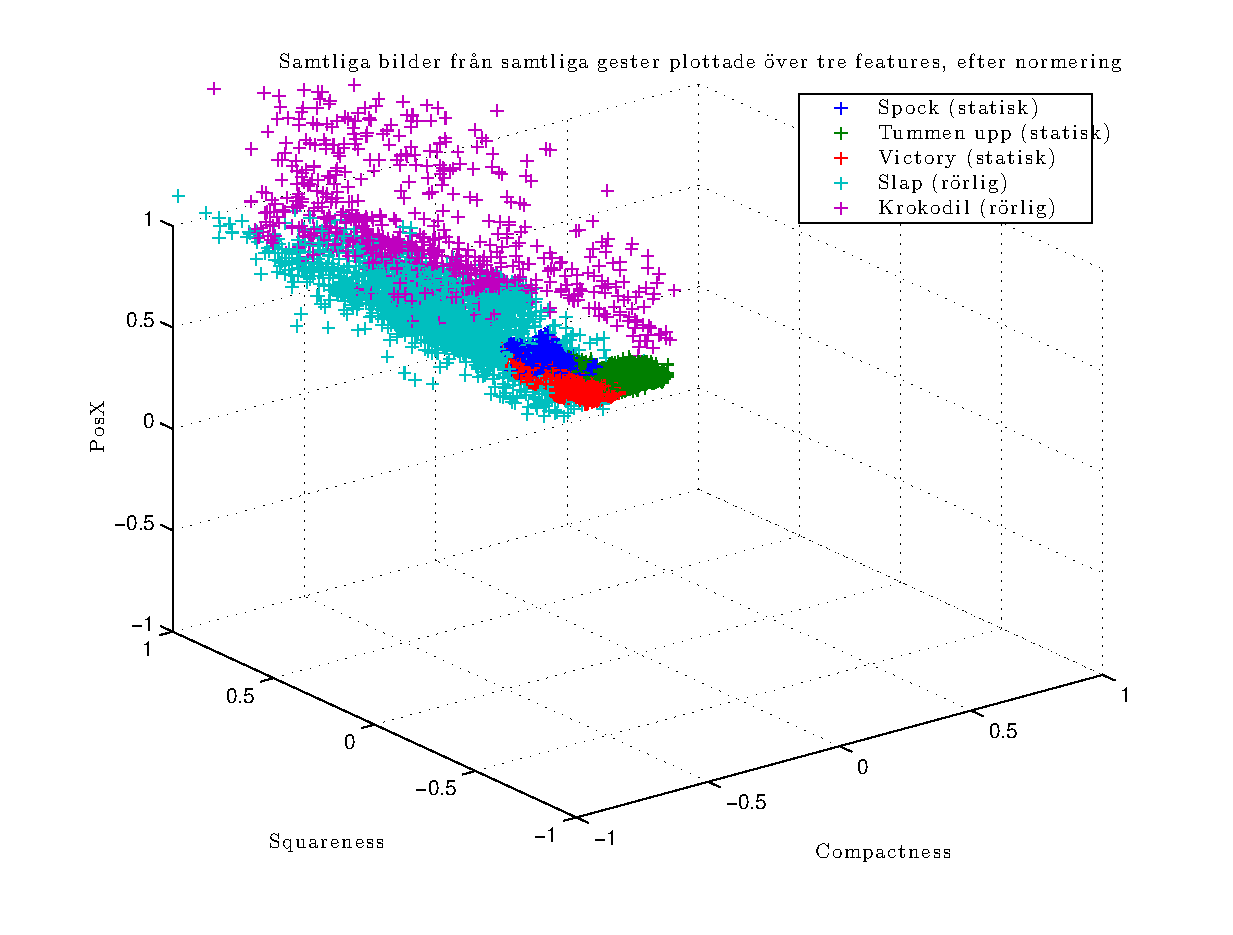
\includegraphics[width=\textwidth]{bilder/feats-1+6+7}
  \caption{De statiska gesterna är betydligt svårare att skilja på än
  de rörliga, vilket illustreras av de tre tydligast grupperande
  egenskaperna.}
  \label{fig:feats167}
\end{figure}

\end{document} 

